\section{わかるらんど}
『わかるらんど』のユーザインタフェースは「ダッシュボード」と「投稿画面」の2つからなり,
画面右上のボタンで切り替えることができる.
図\ref{dashboard}はダッシュボードのスクリーンショットである.
ユーザが投稿したテキストやスタンプや,
各種のセンサのデータなどがリアルタイムに1つの画面に表示されている.
センサのデータなどは自動的に更新され,ユーザのリアクションは図\ref{console}の投稿画面で
ユーザ名を入力し,スタンプを一覧から選んで投稿することで
自分のアイコンの上にオーバーレイ表示される.
ユーザの投稿には表示時間が設定されており,
指定時間が経過すると自動的に投稿が取り下げられるため
いつまでも古い投稿が表示され続けてしまうということはない.

\begin{figure}[h]
\centering
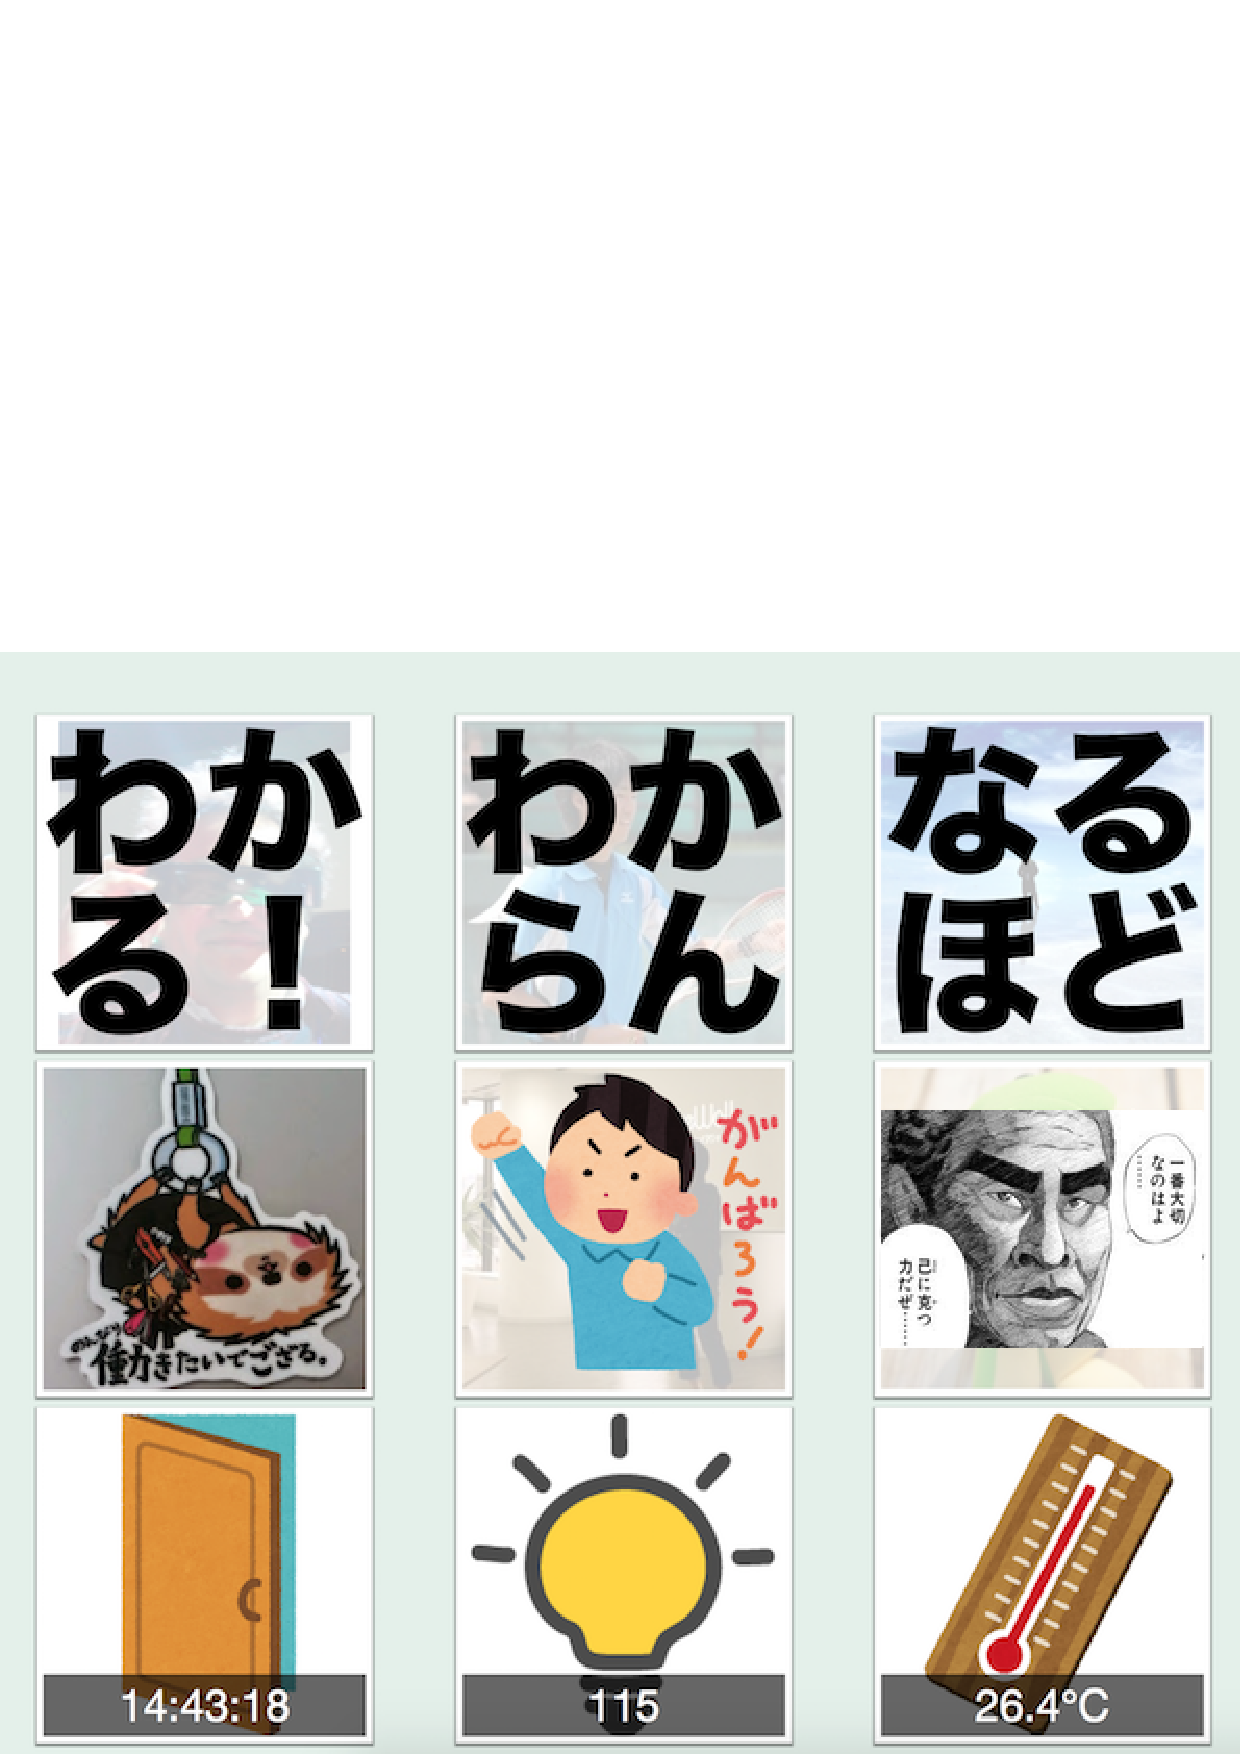
\includegraphics[width=6cm]{images/dashboard.png}
\caption{『わかるらんど』のダッシュボード}
\label{dashboard}
\end{figure}

\begin{figure}[h]
\centering
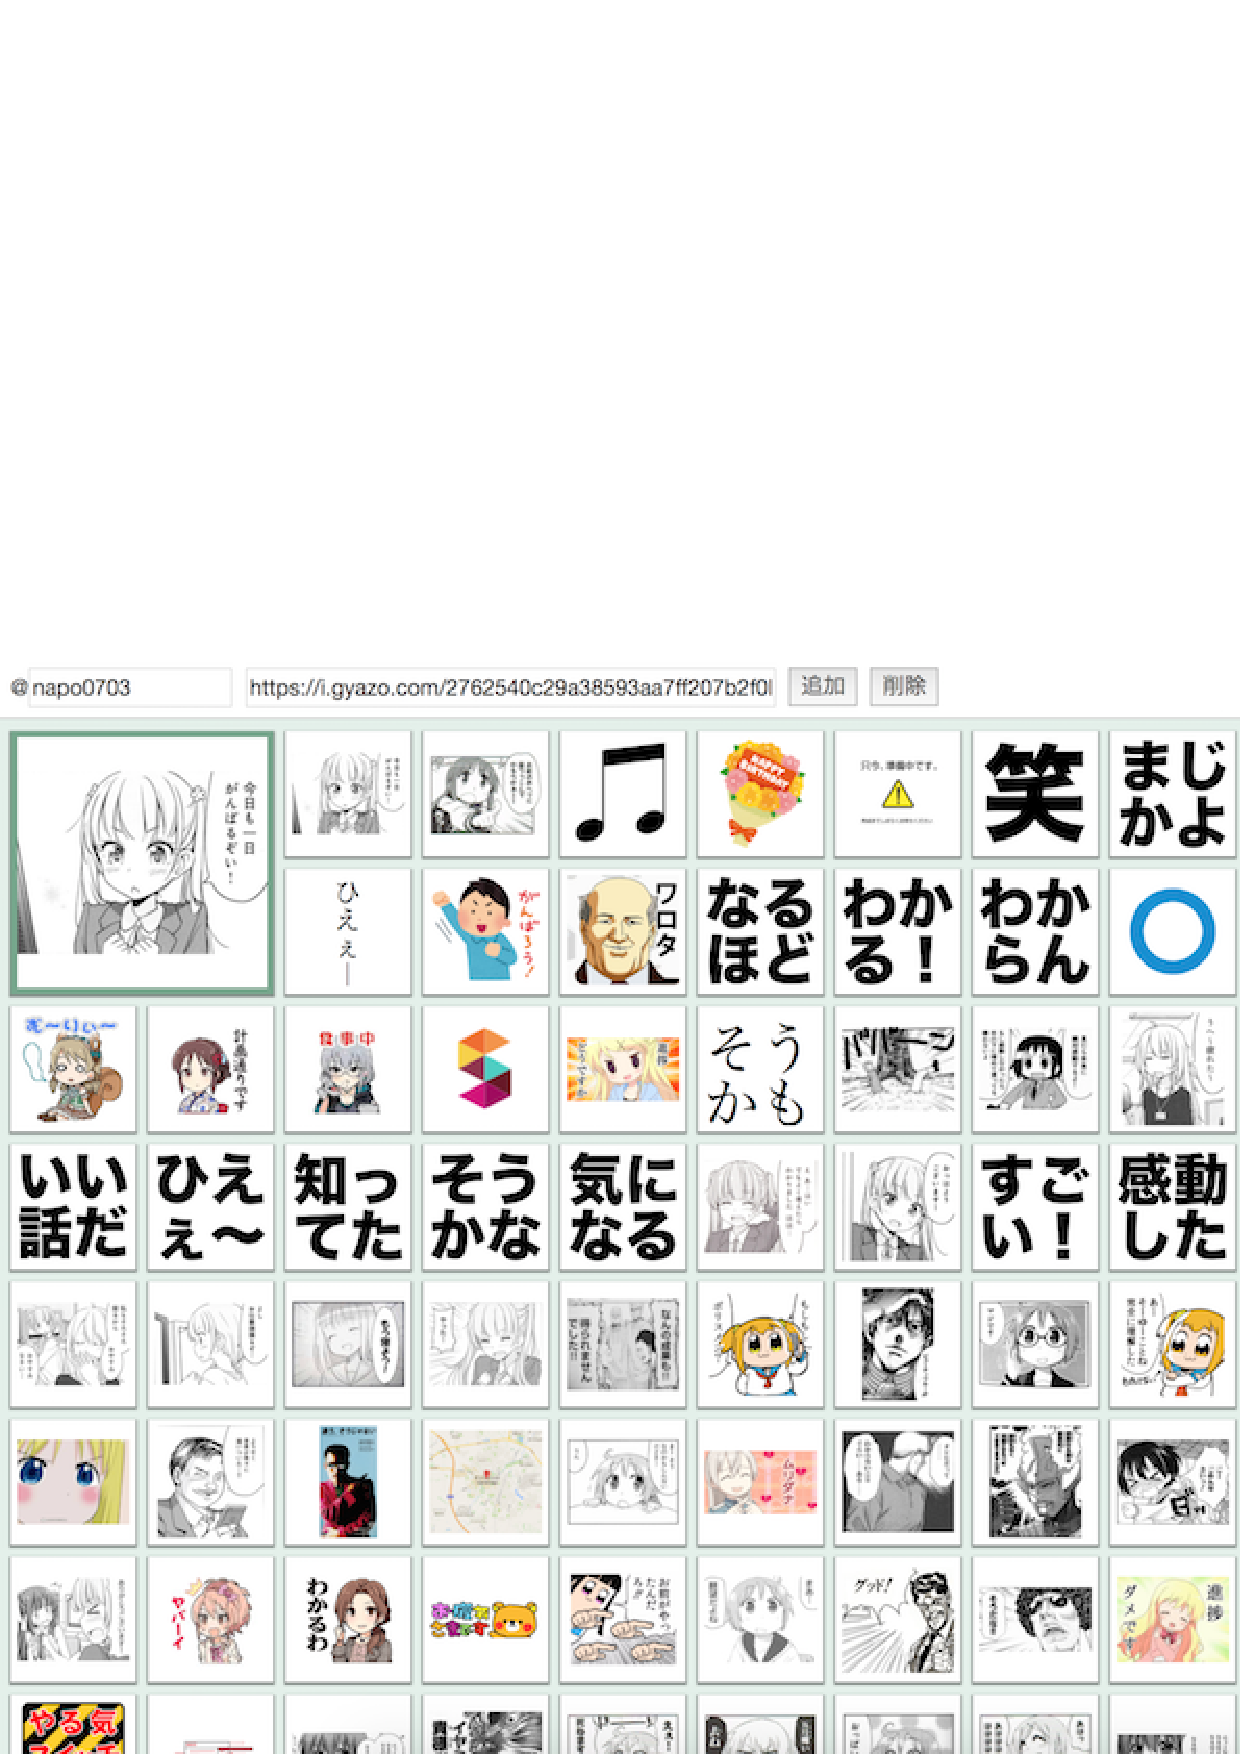
\includegraphics[width=6cm]{images/console.png}
\caption{『わかるらんど』の投稿画面}
\label{console}
\end{figure}